\section{Predicate Exchange}
% zenna-todo: Why do we need predicate exchange?

To condition a model $\cM$ on a predicate $Y$ we develop \emph{predicate exchange}, a likelihood-free inference procedure.  It is composed of two parts:
\begin{enumerate}
\item \textbf{Predicate Relaxation} constructs a soft predicate $\softv{Y}$ from $Y$. $\softv{Y}$ takes values   in a soft Boolean algebra: the unit interval $[0, 1]$ with continuous logical connectives $\soft{\land}$. $\soft{\lor}$ and $\neg$. 
$\softv{Y}$ is 1 iff $Y$ is 1, but otherwise takes nonzero values denoting the degree to which $Y$ is satisfied.
% The relaxation is parameterized by a temperature.
% Predicate relaxation allows us to apply likelihood based MCMC inference procedures.
\item  \textbf{Replica Exchange} is a Markov Chain Monte Carlo procedure that exploits temperature. The strength by which $\softv{Y}$ relaxes $Y$ is modulated by a temperature parameter $\alpha$, which trades off between accuracy and ease of inference.  By simulating several replicas of $\softv{Y}$ at different temperatures, replica exchange is able to draw exact samples. 
\end{enumerate}

% \subsection{Soft Conditioning}
% Conditioning is an operation that restricts a measure space by a set.

% Let $(\Omega, \mathcal{H}, \mathcal{P})$ be a measure space.
% Soft conditioning on a function $Y: \Omega \to [0, 1]$ constructs a new measure $\mathcal{P}'$ defined as:
% \begin{equation}
% \mathcal{P}'(A) = \frac{\mathbb{E}(Y \mid A)}{\mathbb{E}(Y)}
% \end{equation}

\subsection{Predicate Relaxation}\label{predexchange}

A soft predicate $\softv{Y}$ approximates $Y$ in the sense that when viewed as a likelihood function on model parameters, $\softv{Y}$ has a broader support, assigning nonzero weights to parameter values which have zero weight under $Y$.
There are three desiderata which govern this approximation.
First, $\softv{Y}$ should have a temperature parameter $\alpha$ that controls the fidelity of the approximation. In particular, $\softv{Y}$ should converge to $Y$ as $\alpha \to 0$, and to a flat surface as $\alpha \to \infty$. Second, the fidelity of the approximation should vary monotonically with temperature. Third, $\softv{Y}$ should be consistent with $Y$ on 1. That is $Y(\omega) = 1$ iff $\softv{Y}(\omega) = 1$ at all temperatures.  


% The family of approximations of the predicate $Y$ is parameterized through a temperature $\alpha$ that controls the smoothness of the approximation. In particular, $\softv{Y}$ with $\alpha \to 0$ converges to $Y$ itself while increasing values of $\alpha$ yield smoother approximations eventually giving a flat surface when $\alpha \to \infty$. Moreover, the set of conditional samples $C(Y) = \{ \omega \in \Omega \text{ } | \text{ } Y(\omega) = 1 \}$ are assigned a value of $1$ in $\softv{Y}$ for all temperatures. 

% To construct a $\softv{Y}$ with such properties, we let $Y$ be the following predicate $a=b$ for standard Gaussians $a, b \sim \mathcal{N}(0, 1)$. We choose a distance
% $\rho(a, b)$ to indicate how close our sample is to $C(Y)$. To meet the desiderata
% of having $C(Y)$ be $1$ over the constraint set and to ensure the constraint becomes
% smoother with large $\alpha$, we use a function $k : [0, \infty] \to [0, 1]$ parameterized by $\alpha$ to wrap the distance $\rho(a, b)$. A simple choice for such a function is $k(d; \alpha) = e^{-d / \alpha}$ that provides the desired properties to $\softv{Y}$ (see Appendix). The formal definition of $\softv{Y}$ is as follows.

\begin{definition}
A function $\softv{Y} : \Omega \to [0, 1]$ parameterized by $\alpha \in [0, \infty)$ is a relaxation of $Y: \Omega \to \{0, 1\}$ if:
\begin{enumerate}[label=(\roman*)]
	\label{def:temp}
	\item For all $\omega \in \Omega$, $\lim_{\alpha \to 0}\softv{Y}(\omega; \alpha) = Y(\omega)$.
	\item For all $\omega \in \Omega$, $\lim_{\alpha \to \infty}\softv{Y}(\omega; \alpha) = 1$.

    \item For all $\alpha$, $\softv{Y}(\omega; \alpha) = 1$ iff $Y(\omega) = 1$.
    \item The entropy $H(\softv{Y}(\omega; \alpha))$ (which characterizes the fidelity of the approximation ) is an increasing function of $\alpha$.\footnote
    {By compactness, it is integrable for all $\alpha$, when $\Omega$ has finite dimension}
\end{enumerate}
\end{definition}

\paragraph{Graded Satisfiability}
$\soft{\lk}_{\inf}(m)$ represents the degree to which a model realization $m$ satisfies a predicate.
Let $k_\alpha$ be a kernel (described below), $\rho$ a distance metric, and $A = \{(x_1, \dots, x_n) \mid \lk(x_1, \dots, x_n) = 1\}$ the satisfying set.
$\soft{\lk}_{\inf}(m)$ is then:
\begin{equation}
\soft{\lk}_{\inf}(m) = k_\alpha(\rho(m, A))
\end{equation}
where $\rho(x, A) = \inf \left\{\rho(x, a) \mid a \in A\right\}$.
% As shown in the Section \ref{implement}, $\soft{\lk}_{\inf}$ can be difficult to compute.

\paragraph{Distance} A relaxation kernel $k_\alpha$ bounds distances from $\rho$ to the unit interval, and is paramterized by temperature $\alpha$.
% For example if $x$ and $y$ are real values, then $x \soft{=} y$ is defined as $k_\alpha(\rho(x, y))$ where $\rho$ is a distance function and $k_\alpha$ is a relaxation kernel paramterized by temperature $\alpha$.
% A relaxation kernel maps distances to values in $[0, 1]$, and ensures that $\softv{Y}$ adheres to the outlined criteria.
We restrict our attention to the squared exponential kernel:
\begin{equation}
k_{\alpha}(r) = \exp\left(-\frac{r^2}{\alpha}\right)
\end{equation}

$\rho$ is parameterized by the type of input.
For canonical spaces such as $\mathbb{R}$ and $\mathbb{N}$ we default to the Euclidean distance. 
$x \soft{=} y$ is then defined as $\exp(\norm{x - y}/\alpha)$.
For composite elements $x, y \in \mathbb{T}_1 \times \cdots \times \mathbb{T}_n$ of product type, by default $\rho$ takes a mean $\rho(x, y) = (1/n)\sum^n_{i=1}\rho(x_i, y_i)$.



  % \begin{center}
  % \begin{tabular}{ c |  c | c }
  %   \hline		
  %   $x \soft{=} y$ & $x \soft{>} y$ & $x \soft{<} y$  \\
  %   $k_\alpha(\rho(x, y))$ & $k_\alpha(\rho(x, [y, \infty]))$ & $k_\alpha(\rho(x, [-\infty, y]))$ \\
  %   \hline  
  % \end{tabular}
  % \end{center}



\paragraph{Composition} We construct $\softv{Y}$ from $Y$ compositionally, by substituting primitive predicates (equality, inequalities and logical operators) with soft counterparts.
For instance the predicate $(x > y) \lor \neg(x^2 = 2)$ is transformed into $(x \soft{>} y) \soft{\lor} \softv{\neg}(x^2 \soft{=} 2)$.
In general, we use $\soft{p}$ to denote a relaxation of a predicate $p$.
\begin{figure}[H]\label{softpreds}
  \begin{align*}
x \soft{=} y &= k_\alpha(\rho(x, y))\\
x \soft{>} y &= k_\alpha(\rho(x, [y, \infty]))\\
% x \soft{<} y &= k_\alpha(\rho(x, [-\infty, y]))\\
x \soft{<} y &= k_\alpha(\rho(y, [-\infty, x]))\\
a \soft{\land} b &= \max(a, b)\\
a \soft{\lor} b &= \min(a, b)
\end{align*}
\caption{Soft Primitive Predicates}
\end{figure}

A soft inequality such as $x \soft{>} y$ is function of the amount by which $x$ must be increased (or $y$ decreased) until $x > y$ is true.
This is the distance between $x$ and the interval $[y, \infty]$, where the distance between a point and any interval $[a, b]$ is the smallest distance between $x$ and any element in $[a, b]$, and therefore 0 if $x \in [a, b]$:
\begin{equation}
\rho(x, [a, b]) =
\begin{cases}
  a - b & \text{ if } x < a\\
  x - b & \text{ if } x < b\\
  0              & \text{otherwise}
\end{cases}
\end{equation}

Soft negation introduces complications.
To illustrate, Figure \ref{negationimg} (a) shows $x \soft{>} 0$ as a function of $x$.
In continuous logics \cite{kimmig2012short}, the negation of $a \in [0, 1]$ is $1 - a$.
However, as shown in Figure \ref{negationimg} (b), this violates criteria (iii) of predicate relaxation; there are values which satisfy the hard predicate $\neg(x > 0)$ which do take a value of 1 in $1 - (x \soft{>} 0)$.


\begin{figure}
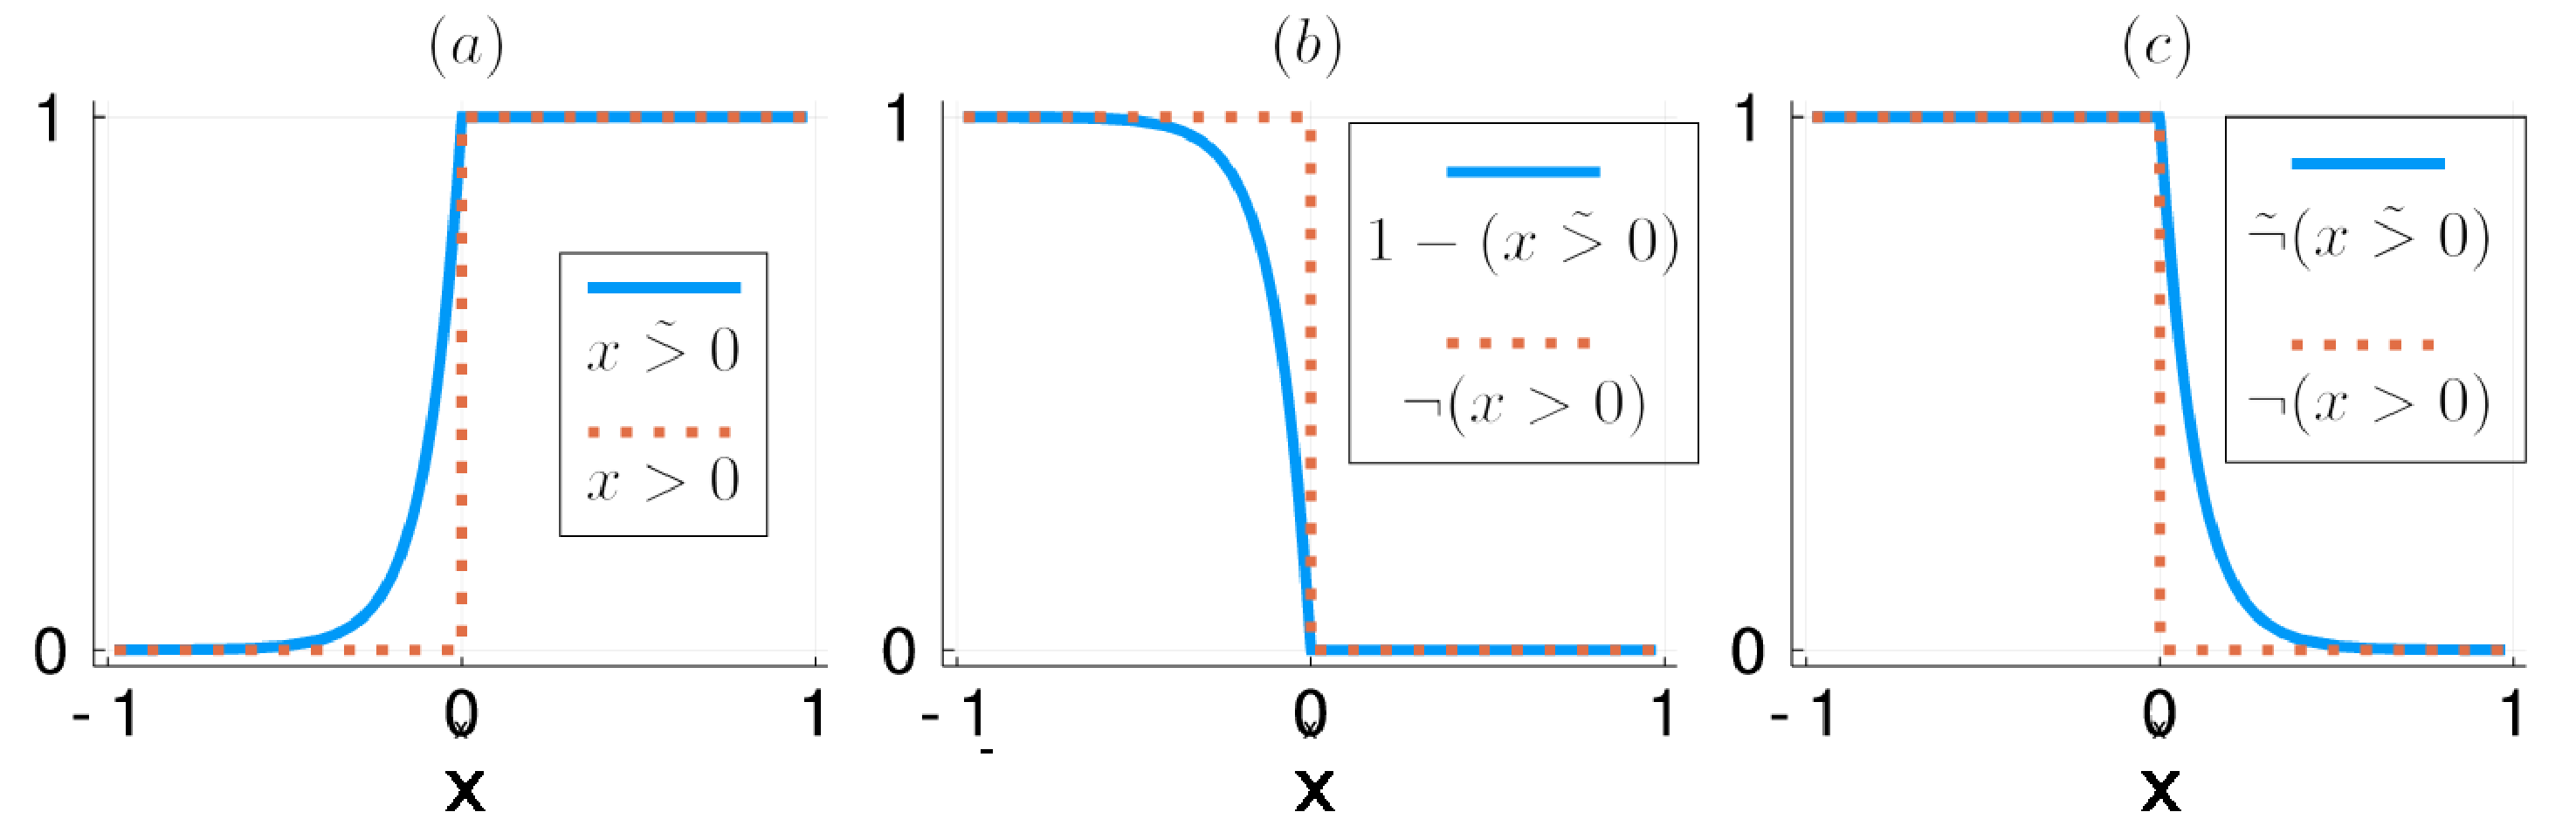
\includegraphics[width=\linewidth]{negation.eps}
\caption{Soft predicates as function of $x$.  In all figures the blue line denotes the soft predicate, while the red line denotes the predicate to approximate.}\label{negationimg}
\end{figure}


The problem of negation arises because $\softv{Y}$ is consistent with $Y$ at 1 but not at 0.
In other words, $\softv{Y}$ is a one-sided approximation.
To overcome this challenge, soft primitives yield a pair $(a_0, a_1)$ where $a_0, a_0 \in [0, 1]$.
$a_1$ preserves consistency with $Y$ on $1$, just as before, while $a_0$ preserves consistency with $\neg Y$ on $1$.
For example if $x \dsoft{>} 0 = (a_0, a_1)$, then as a function of $x$, $a_0$ and $a_1$ correspond to Figure \ref{negationimg} (a) and (c) respectively.

A complete two-sided soft logic is shown in Figure \ref{softw}.
Although a two-sided predicate has two components, for the sake of conditioning we are still concerned only with the true side $a_1$ in the pair $(a_0, a_1)$.
Soft negation simply swaps the elements of $(a_0, a_1)$ to yield $(a_1, a_0)$.

% \begin{definition}
% The function $\softv{Y} : \Omega \to [0, 1]^2$ parameterized by $\alpha \in [0, \infty)$ is a two-sided relaxation of a $Y: \Omega \to \{0, 1\}$ if:
% \begin{enumerate}[label=(\roman*)]
% 	\label{def:temp}
% 	\item For all $\omega \in \Omega$, $\lim_{\alpha \to 0}\softv{Y}(\omega; \alpha) = (\neg Y(\omega), Y(\omega))$.
% 	\item For all $\omega \in \Omega$, $\lim_{\alpha \to \infty}\softv{Y}(\omega; \alpha) = (0, 1)$.

%     \item For all $\alpha$, $\softv{Y}(\omega; \alpha) = 1$ iff $Y(\omega) = 1$.
%     \item The entropy $H(\softv{Y}(\omega; \alpha))$ (which characterizes the fidelity of the approximation ) is an increasing function of $\alpha$.\footnote
%     {By compactness, it is integrable for all $\alpha$, when $\Omega$ has finite dimension}
% \end{enumerate}
% \end{definition}


\begin{figure}
\begin{align*}
x \dsoft{=} y &= (\text{if } x = y  \text{ then } \exp(1/\alpha) \text{ else } 1, k_\alpha(\rho(x, y)))\\
x \dsoft{>} y &= (k_\alpha(\rho(x, [-\infty, y])), k_\alpha(\rho(x, [y, \infty])))\\
x \dsoft{<} y &= (k_\alpha(\rho(y, [x, \infty])), k_\alpha(\rho(y, [-\infty, x])))\\
(a_0, a_1) \dsoft{\land} (b_0, b_1) &= (a_0 \soft{\land} b_0, a_1 \soft{\land} b_1)\\
(a_0, a_1) \dsoft{\lor} (b_0, b_1) &= (a_0 \soft{\lor} b_0, a_1 \soft{\lor} b_1)\\
\softv{\neg}(a_0, a_1) &= (a_1, a_0)
\end{align*}
\caption{Two sided soft primitive predicates}
\label{softw}
\end{figure}

% \begin{center}
% \begin{tabular}{ l | c | r }
%   % \hline		
%   $(a_0, a_1) \soft{\land} (b_0, b_1)$ & $(a_0, a_1) \soft{\lor} (b_0, b_1)$ & $\neg(a_0, a_1)$ \\
%   $(a_0, a_1) \soft{\land} (b_0, b_1)$ & $(a_0, a_1) \soft{\lor} (b_0, b_1)$ & $\neg(a_0, a_1)$ \\
%   % \hline  
% \end{tabular}
% \end{center}


\paragraph{Unsatisfiability}Predicate exchange is unable to determine if a predicate is unsatisfiable (e.g.  $(x > 1) \land (x < -1)$), and defers to the user to ensure this is the case.

\subsection{Approximate Markov Chain Monte Carlo}
A soft predicate can serve as an approximate likelihood, and as a result is amenable to likelihood based inference methods such as Markov Chain Monte Carlo.
MCMC algorithms require a function $f$ that is proportional to the the target density.
In Bayesian inference this is the posterior, dictated by Bayes' theorem as the product of the likelihood and the prior.
Approximate inference using soft predicates takes a similar form.

Let $\cM = (X_1, \dots, X_n)$ be a model, $Y$ be a predicate that conditions $\cM$, and  $\softv{Y}(\omega) = \softv{\lk}(X_1(\omega), ..., X_n(\omega))$ be a relaxation of $Y$.
% % Random variables in $\cM$ may be exogenous or endogenous in the sense that
% % given values for exogenous variables, the values of endogenous are determined.
% % For example $X = \mathcal{N}(0,1)$ is exogenous while $Y = X^2$ is endogenous.
% % Inference need only take place on exogenous random variables.
% Both $Y$ and $\softv{Y}$ are random variables, and hence map from the sample space $\Omega$;
% for convenience we define a soft predicate $\softv{\lk}$ as a function of its parameters (other random variables in the model) rather than the sample space.
% That is, let $\softv{Y}(\omega) = \softv{\lk}(X_1(\omega), ..., X_n(\omega))$, where $X_i \in \cM$.
Assuming a prior density $p$, the approximate posterior $f$ is the product:
\begin{equation}
f(m) = p(m) \cdot \softv{\lk}(m)
\end{equation}
$\softv{\lk}$ down weights parameter values which violate $Y$ by the degree to which they violate it. 
This is modulated by the temperature $\alpha$ used in the  relaxation kernels which constitute $\softv{\lk}$.
At maximum temperature $\softv{\lk}$ has no effect, and the approximate posterior $f$ is equal to the prior $p$.
At zero temperature, $f$ recovers the true posterior since parameter values which violate the condition are given zero weight.

For illustration, let $\cM = (\mu, X)$ be a model where $\mu = \beta(3, 4), X = \mathcal{N}(\mu, 1)$  conditioned on $X = 0.5$.
The approximate posterior is shown at different temperatures in Figure \ref{temppost} and defined as:
\begin{equation}\label{approxposterior}
f_\alpha(\mu, x) = \beta_{0,1}(\mu) \cdot \mathcal{N}_{\mu,1}(x) \cdot k_\alpha(\rho(x, 0.5)) 
\end{equation}

\begin{figure}
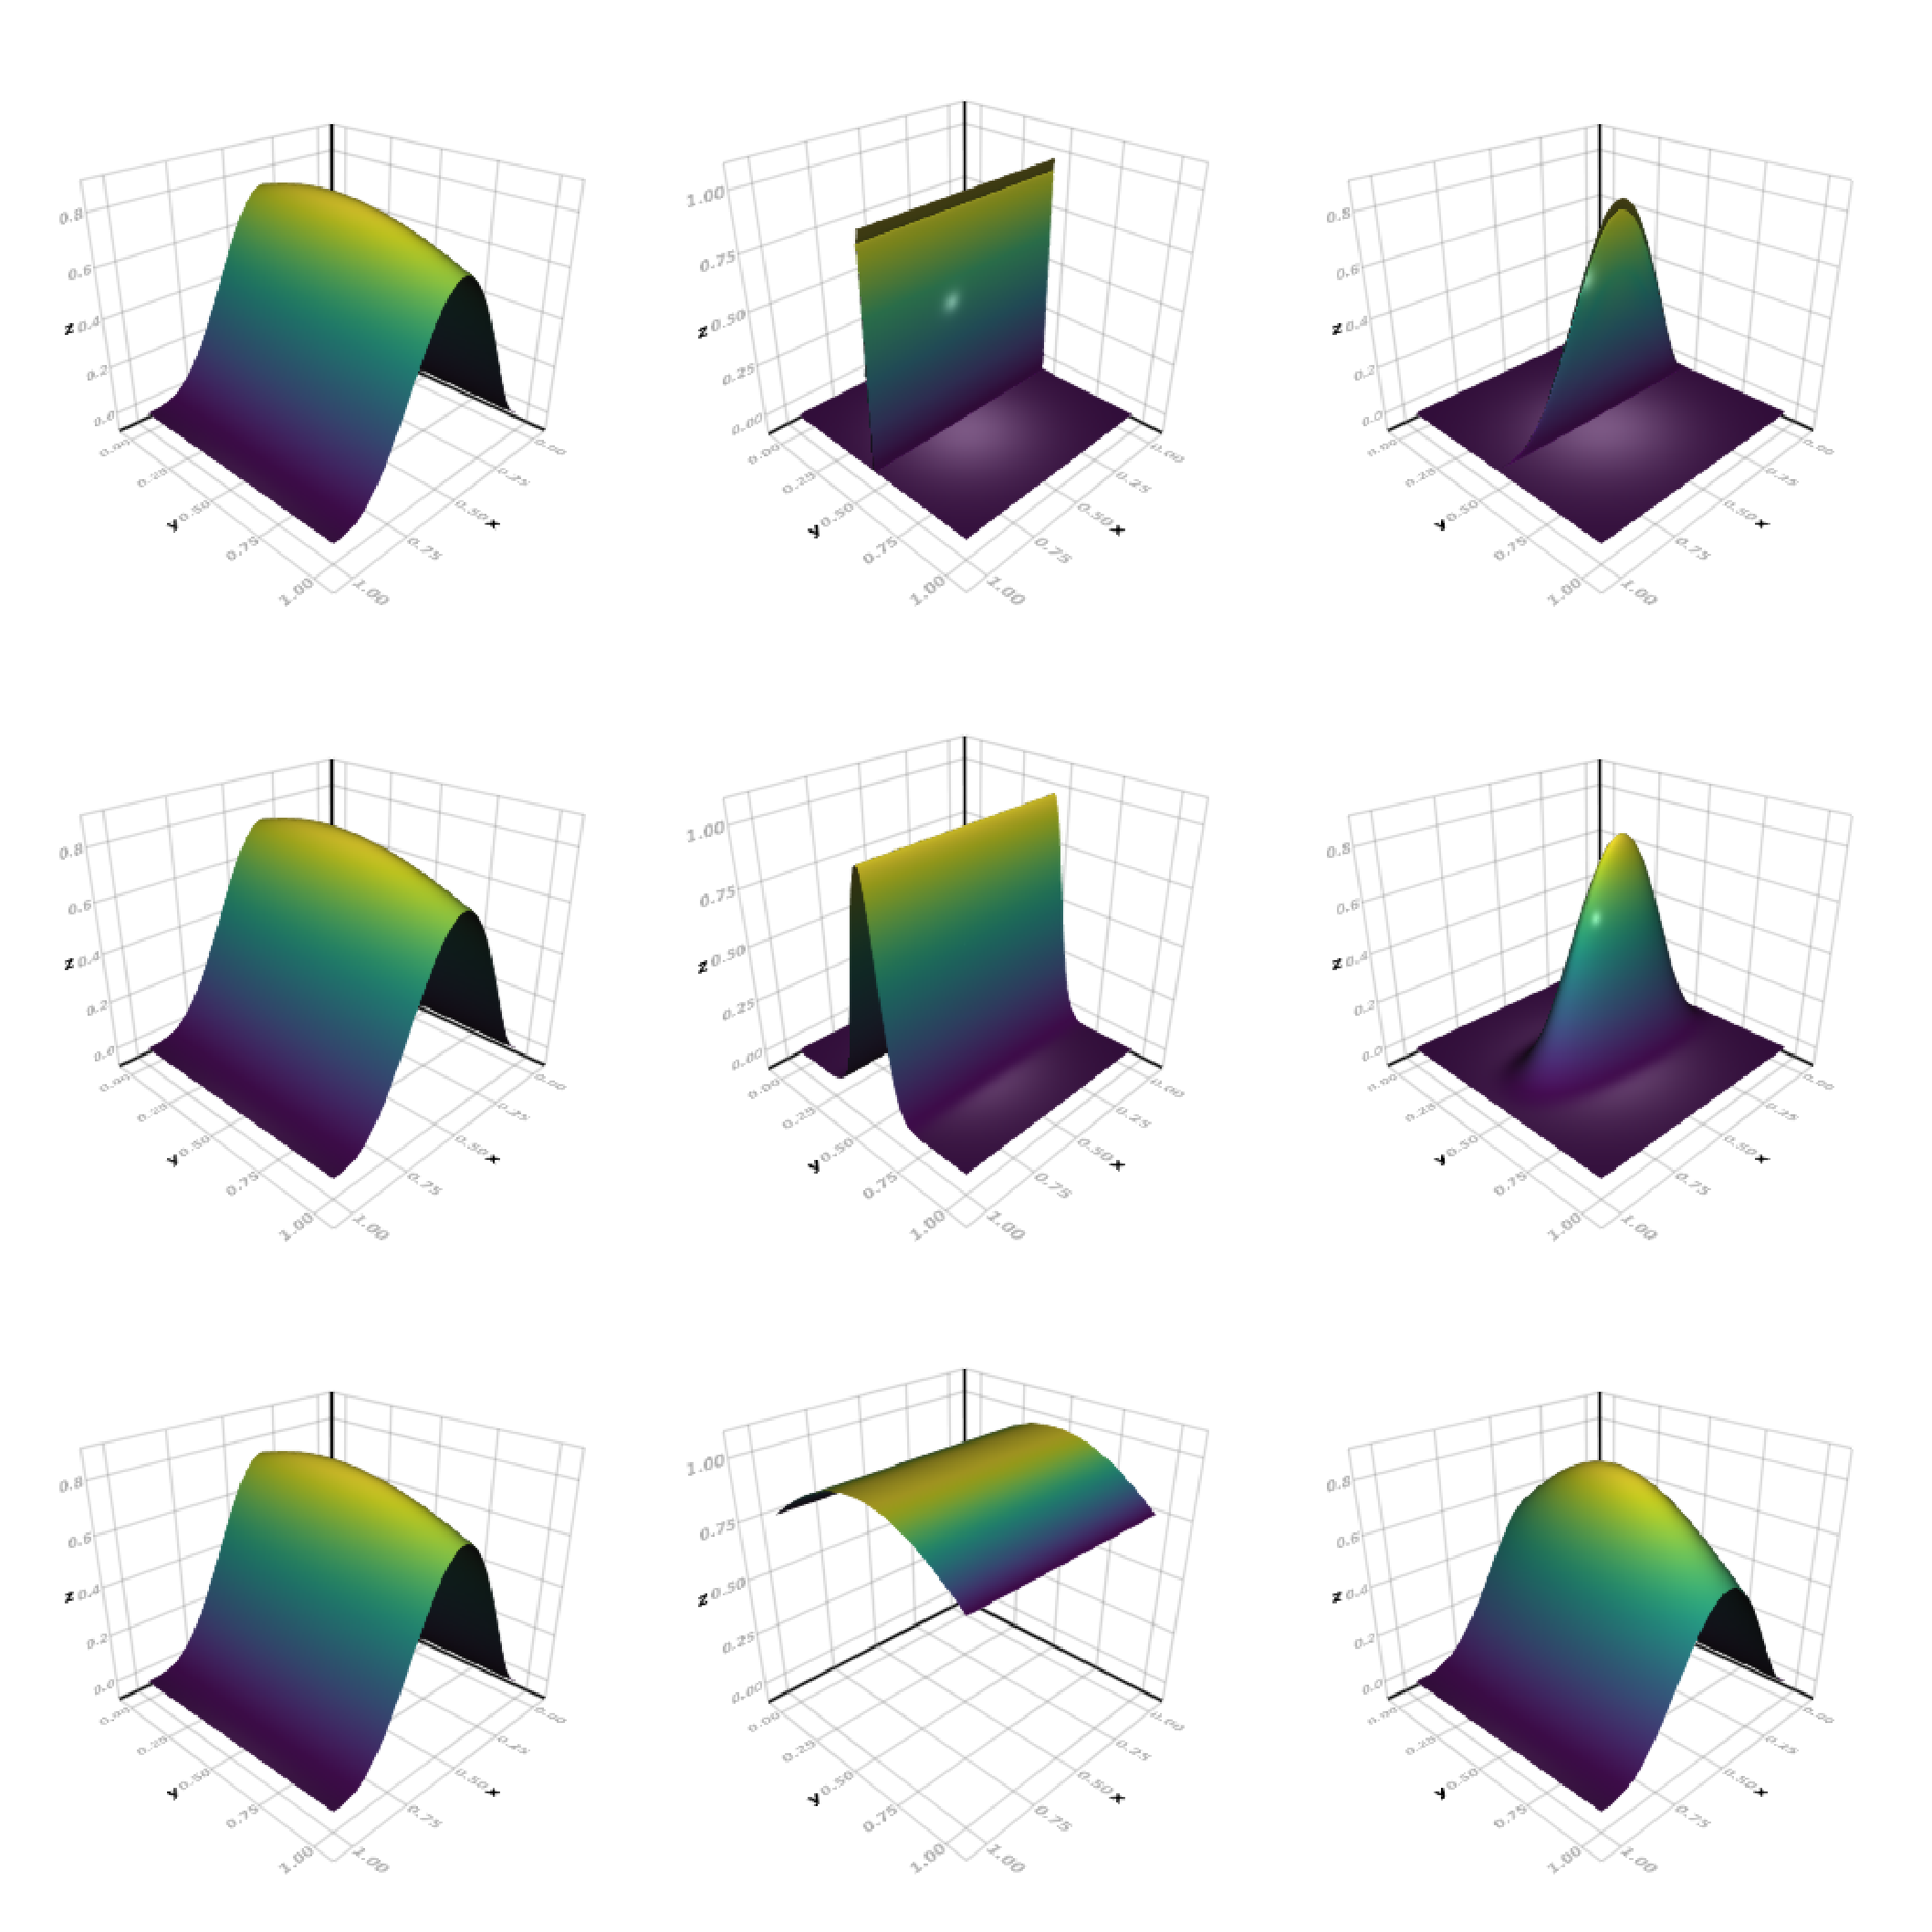
\includegraphics[width=\linewidth]{approxpost.eps}
\caption{Approximate Posterior at varying temperatures.  Temperature decreases from top row to bottom.  Along each row: (left) is the prior term $p$, (center) is the soft likelihood term $\softv{\lk}$, and (right) is the approximate posterior $f$}
\label{temppost}
\end{figure}

The temperature parameter trades off between tractability of inference and the fidelity of the approximation.
Too high and $\softv{Y}$ will diverge too greatly from $Y$. Too low and convergence will be slow.
% Several temperatre methods for controlling temperature exist such as simulated annealing \citep{kirkpatrick1983optimization} and Adiabatic Monte Carlo \citep{betancourt2014adiabatic}.
% We augment replica exchange , which combines information from several chains to sample more effectively, which an accept/reject phase, to sample from the unrelaxed model.

\subsection{Replica Exchange}\label{replicaexchange}
Replica exchange simulates \citep{swendsen1986replica} $M$ replicas at different temperatures, and uses a Metropolis-Hastings update to  periodically swap the temperatures of chains.
If $f_{\alpha_i}$ is an approximate posterior function at temperature $\alpha_i$, two independent parallel chains simulating targets $f_{\alpha_1}(x)$, $f_{\alpha_2}(y)$ they follow a joint target $f_{\alpha_1, \alpha_2}(x,y) = f_{\alpha_1}(x)f_{\alpha_2}(y)$.
Replica exchange swaps states between the chains while preserving the joint target.
Swapping states is equivalent to swapping predicates, which motivates the name predicate exchange.
Concretely, replica exchange proposes a swap from $(x, y)$ to $(y, x)$, and accepts it with probability $\min(1, A)$, where:
\begin{equation}
A =  \frac{f_{\alpha_1, \alpha_2}(y,x)}{f_{\alpha_1, \alpha_2}(x,y)} = \frac{f_{\alpha_1}(y)f_{\alpha_2}(x)}{f_{\alpha_1}(x)f_{\alpha_2}(y)}
\end{equation}

We modify standard replica exchange in two ways: (i) for exact inference, states which violate the constraint are rejected, and (ii)
unlike conventional replica exchange which draws samples only from the zero-temperature chain, we accept states from any chain so long as $f_{\alpha_i}(x) = 1$.

Replica exchange has a number of hyper-parameters: the number of parallel chains, the corresponding temperatures, the swapping schedule.
Several good practices are outlined in \cite{earl2005parallel}.  In practice, we logarithmically space $\alpha$ between a lower and upper bound (e.g., $\log(\alpha_1) = 10^{-5}$, $\log(\alpha_M) = 10^5$), and swap states of chains that are adjacent in temperature ($\alpha_1$ with $\alpha_2$, $\alpha_2$ with $\alpha_3$, etc) periodically.


% \paragraph{Balancing Different Constraints}
% The scales of variables effect their influence on
% the conditional distribution at a fixed temperature.
% For example consider two pairs of variables, where
% the first pair is ten times larger than the second.
% Conditioning on a greater than constraint on both
% pairs of variables is well defined. However,
% a softening of both constraints would have 
% a much larger change in the energy function over
% a standard deviation change in pairs of variables.
% To mitigate this issue, Omega tries enforce equality
% in magnitude between all basic predicates at each temperature.
% % rr: zenna can you add the basic predicates
% To accomplish this, consider the case of two 
% softened predicates $k_1$ and $k_2$. For the
% energy function, Omega introduces a weight
% for all but the first constraint, in this
% case $k_2$ in the energy function gets replaces
% by $\gamma_2 k_2$. The weight $\gamma_2$ should
% ensure that $\gamma_2 k_2$ has the same
% magnitude effect as $k_1$ on the energy
% function:
% \begin{align*}
% E_{p_{\alpha, \gamma_2}}[k_1] = E_{p_{\alpha, \gamma_2}}[\gamma_2 k_2] 
% \end{align*}
% % Does such a gamma_2 always exist? Maybe rewrite it as
% % an optimization problem over gamma to enforce a solution?
% In practice, we set $\gamma_2$ using an exponential moving
% average of the $k_1$ values over the $k_2$ values.


% This scenario closely resembles the reparameterization trick \citep{Kingma:2014, rezende2014stochastic} where one resorts to include all the uncertainty of a random variable $z$ in a simple, easy-to-sample, parameter-free noise source such as $\epsilon \sim \mathcal{N}(\mathbf{0}, I)$. The actual random variable $z$ is then obtained through a parametric transformation of the noise, $z = f(\epsilon; \theta)$. Both methods separate the 
% uncertainty of a random variable from the deterministic transformation that results in a complex density. However, in the reparameterization trick the noise source is constant and controlled while the parametric transformation is meant to infer the structure of the resulting random variable. Conversely, our forward model -- deterministic transformation -- is constant and controlled, hence we simply transfer our inference problem to a much simpler space of $\Omega$.

% Predicate Exchange has a connection to approximate Bayesian computation (ABC) methods~\citep{beaumont2002approximate} in that ABC methods 
% sample using a distance function to induce a data likelihood. Our method differs in that conditionals can be any predicate not just
% one for an observed random variable.
% Finally for inference, with the soft predicates we define, we
% can use modern likelihood-free variational inference algorithms
% that construct an approximation to a conditional with only samples
% from the joint and samples from the conditional approximation~\citep{tran2017hierarchical}.

